\section{ER Diagram}
ER Diagrammet (Ovenstående figur \ref{fig:ER}) viser den logiske model for domænet Min Sundhedsplatform. \\
Entiteterne er de logiske enheder - dvs. aktører, objekter og begivenheder i systemet. 
Relationerne angiver hvilken type af relation, der er mellem entiteterne i systemmet.

Entiteterne angives med rektangler og en tekst typisk et navneord. Til entiteterne er der tilknyttet et eller flere attributter, angivet med en ellipse med en tekst.

Relationerne angives med en diamant med en  tekst, der beskriver relationen mellem to eller flere entiteter.

kardinaliteten beskrives med streger og pile mellem entiteterne. \\ 
En sort lukket pil beskriver: mange til højst en (dvs. 0 eller 1).\\
En åben pil beskriver: mange til præcis en.\\
En streg uden pil beskriver: mange til mange.

Under-entiteter repræsenteres med relationen 'ISA' i en trekant.

En svag entitet er en entitet, der for at relationen kan gælde, kræver at den udover sine egne attributter også skal have sin ejers nøgleattribut som nøgle. Den beskrives med en fed ramme.

Vi kan læse følgende information om Min Sundhedsplatform ud af ER Diagrammet:\\
En patient har tilknyttet attributterne: navn, cpr-nummer, kontakt-info, historik og password/nøglekort. Cpr-nummer er nøgleattribut.\\
Der er en giver-relation fra entiteten patient til entiteten fuldmagt. Der er en mange til en relation, fordi patienten giver fuldmagter og fuldmagterne er givet af én patient. Fuldmagt er en svag entitet, fordi den kræver sin ejers nøgleattribut - dvs. patientens cpr-nummer som nøgleattribut. \\
Patienter har kontakt med mange sundhedsfaglige personer og mange  sundhedsfaglige personer har kontakt ansvar med mange patienter. Læger er under-entitet af sundhedsfaglig personale. \\
Patienten har højest én udbakke, og udbakken tilhører præcis en patient.\\
Patienten har højest én indbakke. Indbakke kan være Påmindelser, Dine Aftaler, Prøvesvar og Spørgeskema.\\
Patienten har højest én journal og en journal tilhører præcis en patient. \\
Journalen har præcis én adgangslog, som har mange logrækker. Logrækken har præcis en adgangslog og præcis en sundhedsfaglig person. En sundhedsfaglig person har mange logrækker.\\
Journalen har én eller ingen diagnose-oversigt og diagnose oversigten tilhører præcis en journal.\\
Journalen har enten ingen eller en journal-notater som tilhører præcis én journal.\\
Journalen har enten én eller ingen målings-oversigt som tilhører præcis én journal.

I designfasen kan den logiske model af ER diagrammet bruges til at danne et overblik over hvilke data, der skal gemmes i systemet, og hvordan flowet er (relationerne mellem entiteterne).\\
ER-diagrammet kan bruges i kommunikationen mellem it-designeren, kunden og brugerne omkring afklaringen af hvilke data, der skal indgå i systemet/domænet. \\
I udviklingsfasen kan ER-diagrammet transformeres til den fysiske model hvor man, ud fra entiteterne, opstiller databaserne/tabeller med de attributter/data, der er behov for i domænet.

\begin{figure}[H]
  \centering
  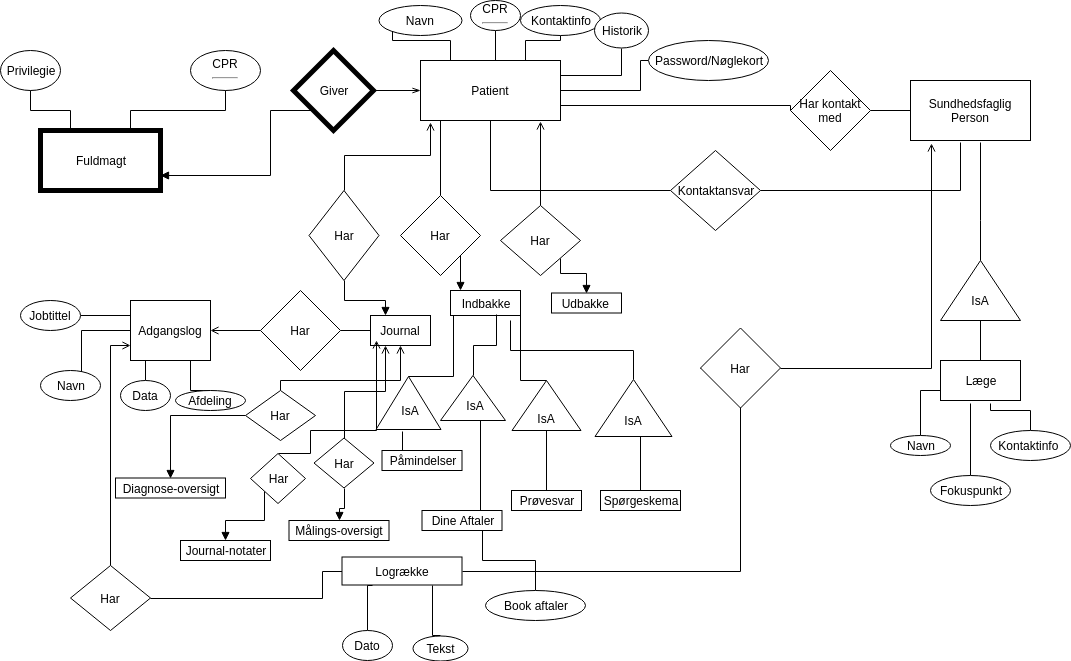
\includegraphics[angle=90, height=0.9\textheight]{Materials/ER-diagram.png}
  \caption{ER-diagram for Min Sundhedsplatform}
  \label{fig:ER}
\end{figure}
